% ****** Start of file .tex ******
%
%   This file is based on apssamp.tex, part of the APS files in the REVTeX 4.1 distribution.
%   Version 4.1r of REVTeX, August 2010
%
%   Copyright (c) 2009, 2010 The American Physical Society.
%   Samuel Balula, Pedro Ribeiro, Luís Macedo, Eduardo Neto 2013
%   See the REVTeX 4 README file for restrictions and more information.
%
% TeX'ing this file requires that you have AMS-LaTeX 2.0 installed
% as well as the rest of the prerequisites for REVTeX 4.1
%
% See the REVTeX 4 README file
% It also requires running BibTeX. The commands are as follows:
%
%  1)  latex filename.tex
%  2)  bibtex filename
%  3)  latex filename.tex
%  4)  latex filename.tex

\documentclass[%
  reprint,
  %superscriptaddress,
  %groupedaddress,
  %unsortedaddress,
  %runinaddress,
  %frontmatterverbose, 
  %preprint,
  %showpacs,preprintnumbers,
  nofootinbib,
  %nobibnotes,
  %bibnotes,
  amsmath,amssymb,
  aps,
  %pra,
  %prb,
  %rmp,
  %prstab,
  %prstper,
  %floatfix,
  10pt,
  a4paper
]{revtex4-1}



\usepackage{facil}                      % Pacote pessoal
\usepackage{verbatim}                   % Apresentação de código
\usepackage{graphicx}                   % Include figure files
\usepackage{dcolumn}                    % Align table columns on decimal point
\usepackage{bm}                         % bold math
\usepackage[latin1,utf8]{inputenc}      % Tipos de caracteres
\usepackage[portuges]{babel}            % Português
\usepackage{indentfirst}                % Identação da primeira linha
\usepackage{hyperref}                   % add hypertext capabilities
\usepackage{float}                      %Fixar imagens
%\usepackage[mathlines]{lineno}          % Enable numbering of text and display math
%\linenumbers\relax                      % Commence numbering lines
%\usepackage[compact]{titlesec}

\usepackage[%showframe,%Uncomment any one of the following lines to test 
%%scale=0.7, marginratio={1:1, 2:3}, ignoreall, % default settings
%%text={7in,10in},centering,
margin=0.5in,        %diminuir margens
%total={6.5in,8.75in}, top=1.2in, left=0.9in, 
includefoot
%height=10in,a5paper,hmargin={3cm,0.8in},
]{geometry}

\begin{document}
\preprint{APS/123-QED}
%\captionsetup[table]{font=small,skip=0pt}
%\captionsetup[figure]{font=small,skip=0pt}
%\titlespacing{\section}{0pt}{*0}{*0}            %Poupar espaço
%\titlespacing{\subsection}{0pt}{*0}{*0}
%\titlespacing{\subsubsection}{0pt}{*0}{*0}


% % % % % % % % % % % % % % % % % % % % % % % % % % % % % % % % % % % % % % % % 
%%%%%%%%%%%%%%%%%%%%%%%%%%%%%%%%%% Início %%%%%%%%%%%%%%%%%%%%%%%%%%%%%%%%%%%%%%
% % % % % % % % % % % % % % % % % % % % % % % % % % % % % % % % % % % % % % % %
 

\title{Levitação magnética com electroiman e fotoresistência}
\thanks{}

\author{Pedro Ribeiro}%
\email{73221, pedro.q.ribeiro@tecnico.ulisboa.pt}
\author{Luis Macedo}%
\email{73633, luis.macedo@tecnico.ulisboa.pt}
\author{Samuel Balula}%
\email{72735, samuel.balula@tecnico.ulisboa.pt}

\affiliation{
  Instituto Superior Técnico\\
  Mestrado em Engenharia Física Tecnológica\\
  Complementos de Electrónica
}

%\collaboration{Grupo 57}

\date{\today}

%%%%%%%%%%%%%%%%%%%%%%%%%%%%%%%%%% Abstract %%%%%%%%%%%%%%%%%%%%%%%%%%%%%%%%%%%%
\begin{abstract}
Neste trabalho laboratorial implementa-se um sistema de controlo que mantem em levitação um objeto metálico não magnetizado.
......................................
#1


\end{abstract}
\maketitle


%%%%%%%%%%%%%%%%%%%%%%%%%%%%%%%%%% Introdução %%%%%%%%%%%%%%%%%%%%%%%%%%%%%%%%%%
\section{Introdução}
\label{s:intro}
%Situar o problema, incluir fórmulas.
%Quem lê o relatório deve conseguir perceber exatamente o que foi feito.
#2

%%%%%%%%%%%%%%%%%%%%%%%%%%%% Experiência realizada %%%%%%%%%%%%%%%%%%%%%%%%%%%%%
\section{Experiência Realizada}
\label{s:expreal}
%Incluir diagrama de blocos da montagem
De acordo com as instruções do guia, implentou-se o circuito da \rfig{../img/esquematico.png}. Apresentam-se na tabela \ref{partlist} os componentes utilizados.

\figurao{../img/esquematico.png}{Circuito implementado no laboratório}

\tabela[partlist]{Lista dos componentes utilizados}{lrrr}{
	Descrição		&Modelo/Valor		&Qt.			&Referência	\\ \hline
	Ampl. operacional	&			&1			&		\\
	Cond. cerâmico		&nF			&1			&		\\
	Resistência .25W	&$\Omega$		&4			&		\\
	#3
}

Para facilidade de análise, divide-se o circuito nas suas partes constituintes, que se analisam separadamente.

\subsection{LED}
%4
	
	
	
	
\subsection{Divisor de Tensão}
%Da a tensao de referencia
%5







\subsection{Fotoresistência}
%6
Uma fotoresistência é um componente composto por um material que sofre variação da sua resistividade com a variação da intensidade da luz incidente neste (também conhecido como fotocondutividade).\\
O dispositivo utilizado sofria um aumento da sua condutividade (e consequentemente uma diminuição da resistência) com o aumento da intensidade luminosa. Integrando este dispositivo num divisor de tensão, como se mostra na figura \ref{fig:foto_res}, que obedece à relação:
\begin{equation}
V_{out}=\frac{R_3}{R_3+R_4}V_{in}
\label{eq:div_t}
\end{equation}
\begin{figure}
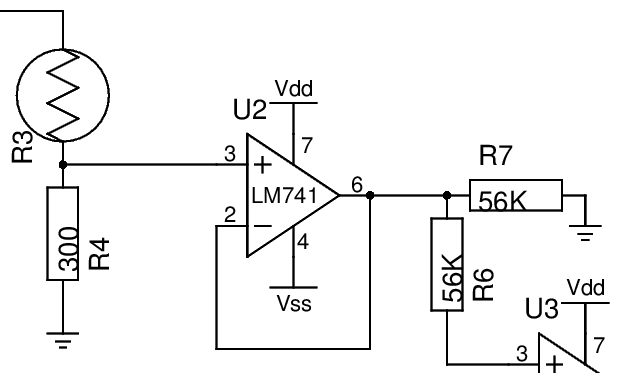
\includegraphics[width=3in]{../img/sensor.png}
\caption{Esquemático do divisor de tensão de tensão onde se inseriu o sensor ($R_3$) com seguidor de tensão.}
\label{fig:foto_res}
\end{figure}
Desta forma, e de acordo com a relação obtida em \ref{eq:div_t}, o sinal de saída do divisor de tensão será tanto maior quanto maior for a resistência $R_3$, ou seja, quanto menor for a intensidade da luz incidente no sensor.\\
Coloca-se um seguidor de tensão em série com a saída do divisor de tensão para minimizar a impedância de saída deste.


\subsection{tensão de referência}
%7






\subsection{Somador integrador}
%8







\subsection{Amplificador não inversor}
%9









\subsection{Rectificação}
%10






\subsection{Andar de saída em classe B}
%11



%%%%%%%%%%%%%%%%%%%%%%%%%%%%%%%% Resultados %%%%%%%%%%%%%%%%%%%%%%%%%%%%%%%%%%%%
\section{Resultados}
\label{s:resul}
%incluir tabelas. Excesso de dados => grafico com valores mais significativos
%12







%%%%%%%%%%%%%%%%%%%%%%%%%%% Análise dos resultados %%%%%%%%%%%%%%%%%%%%%%%%%%%%%
\section{Análise de resultados}
\label{s:aresul}
%Proponho eliminar.... (sam)





%%%%%%%%%%%%%%%%%%%%%%%%%%% Conclusões e Críticas %%%%%%%%%%%%%%%%%%%%%%%%%%%%%%
\section{Conclusões e Críticas}
\label{s:conclu}
%Incluir melhorias propostas à experiência
%13





%\begin{acknowledgments}
%\end{acknowledgments}

%%%%%%%%%%%%%%%%%%%%%%%%%%%%%%%%%%%%%%%%%%%%%%%%%%%%%%%%%%%%%%%%%%%%%%%%%%%%%%%%
% % % % % % % % % % % % % % % %     FIM    % % % % % % % % % % % % % % % % % % % 
%%%%%%%%%%%%%%%%%%%%%%%%%%%%%%%%%%%%%%%%%%%%%%%%%%%%%%%%%%%%%%%%%%%%%%%%%%%%%%%%

\nocite{*}
\bibliography{bibliografia}{}
\bibliographystyle{plain}% Produces the bibliography via BibTeX.
\end{document}
%end of file
